\chapter{Genetic Algorithm}
\label{chapter:intro}
\section{遺傳演算法(Genetic Algorithm, GA)介紹}
遺傳演算法是一種從遺傳科學中獲得啟發的技術,目前被廣泛應用於解決優化問題,尤其在特徵篩選方面引起。在GA中通常使用染色體的概念作為解決方案,通常基因數與特徵數箱等,例如Z=(0,1,1,0,1,0,0,0)代表一染色體上共有8個特徵,1則代表以選擇特徵;0則代表未選擇特徵。
GA主要由三種運算組成,分別為親代選擇、交叉與突變。首先生成具有隨機染色體集合的初始群集,之後評估每個染色體的適合度,並從中基於適合度的概率來選擇親代父母,接下來在親代父母之間進行交叉,生成從親代父母繼承基因的染色體特徵子集,此外根據突變率可能導致生成的染色體子集突變(即0變1或是1變0),之後評估新生成的染色體子集適合度,並將新生成的染色體子集加入當前的群集中,並根據適合度進行排序,選擇最佳的N條染色體應用於下一代,重複該算法直到設定的最大迭代次數為止,最後選擇全局最佳染色體作為最佳特徵子集。
\begin{figure}[H]
	\centerline{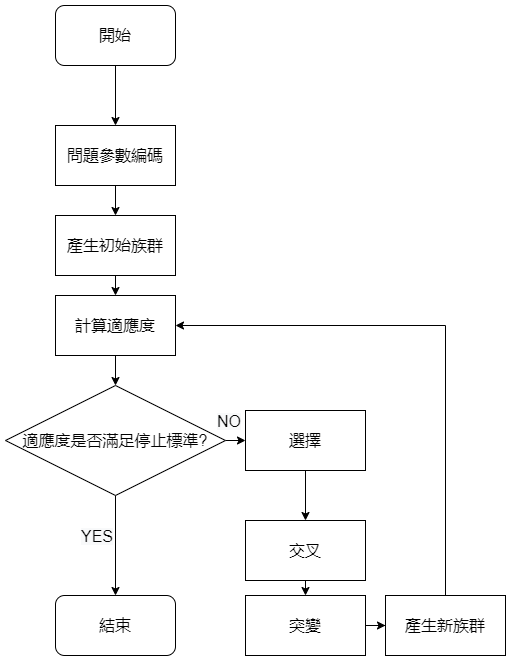
\includegraphics[height=8cm]{pic/GAprocess .png}}
	\caption{GA流程圖}
	\label{fig:GApro}
\end{figure}

\label{sec:background}
\section{適應度(Fitness)計算}

在每完成初始族群取選後,須針對所有被選取的個體,計算其適應能力,做為接下來選種的依據, 每一個個體都被評估後得到一個適應能力值,族群中的個體被按照適應度排序,適應度高的在前面,如果用代價函数(Cost Function)來當評估標準,則需看是要實際問題是要求最大值(Maximum)還是最小值(Minimum)。
\section{親代選擇}
GA使用選擇運算子來對群體中的個體進行優勝劣汰操作:根據適應函數評估出每一個個體的適應度值大小選擇,適應度較高的個體會被挑選 出來複製到下一代群體中的機率較大,適應度低的自然被選出來的機率就較小。 這樣可以使得群體中個體的適應度不斷的往最佳解的方向移動,而不是盲目搜尋。

         \begin{enumerate}
        \item 
       輪盤式選擇(Roulette Wheel Selection):\\
       首先要計算每一個體的適應度,然後計算出此適應度在群體適應度總和中所佔的比例,表示該個體在選擇過程中會被選中的機率,適應度越大被選擇的機率越大。選擇想法就是適應程度越好,所被選擇的機率越大,適應程度越差,所被選擇的機率越小,如此以來,在選擇時適應程度越好的,也越有機會被選中,就如同生物進化過程中的「適者生存,不適者淘汰」的觀念,希望將優良基因會遺傳給下一代的個體。
                \begin{figure}[H]
            \centerline{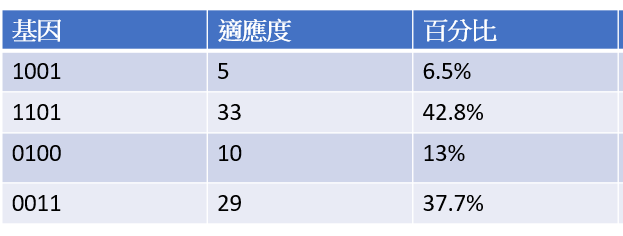
\includegraphics[width=10cm]{pic/Wheel.PNG}}
            \caption{基因編碼與適應度}
            \label{fig:wheel}
        \end{figure}
                 \begin{figure}[H]
            \centerline{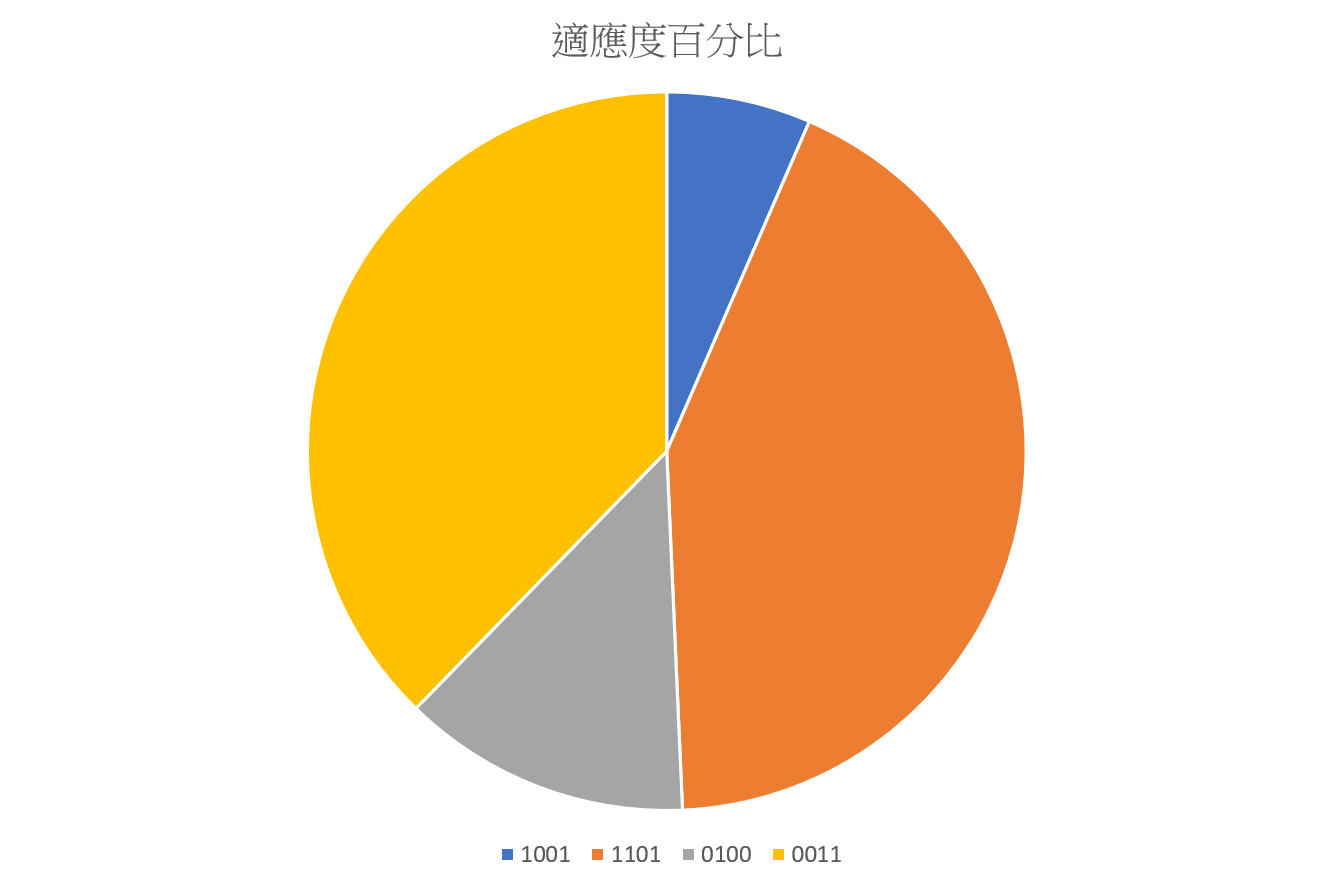
\includegraphics[width=10cm]{pic/wheelFitness.png}}
            \caption{輪盤法適應度百分比圖}
            \label{fig:wheelf}
        \end{figure}
        如果群體的適應度差異巨大時,最佳個體的被選擇機率會大幅成長,容易使這個最佳個體充斥在當前群體中,使得群體喪失多樣性,過早失去進化能力。
       
       \item  
       競爭式選擇(Tournament Selection) 
        競爭式選擇中,按照輪盤選擇的機率為依據,隨機取得幾個基因續列,並立即進行比較,將適應力較好的留下,因為是用機率選取基因,所以不但可以塞選出好基因,也能避免輪盤法則的缺點發生。
        \end{enumerate}

\section{交叉(crossover)}
交叉將兩個父輩染色體上的基因進行重新組合分配,從而產生下一代個體的過程,通過交叉可能會將兩個父輩的優勢基因組合在一起,產生適應度更高、更接近最優解的新個體。

\begin{enumerate}
	\item
	      單點交叉:
	      單點交叉算法就是指定了單個交換點用於父輩的基因交換重組。如圖\ref{fig:one}
	      \begin{figure}[H]
		      \centerline{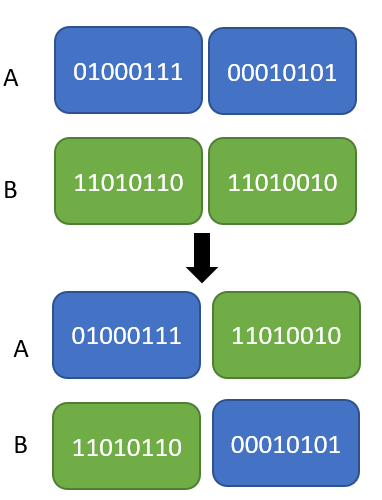
\includegraphics[height=8cm]{pic/one.PNG}}
		      \caption{單點交叉示意圖}
		      \label{fig:one}
	      \end{figure}

	\item
	      多點交叉:
	      多點交叉算法就是指定了多個交換點用於父輩的基因交換重組。如圖\ref{fig:two}
	      \begin{figure}[H]
		      \centerline{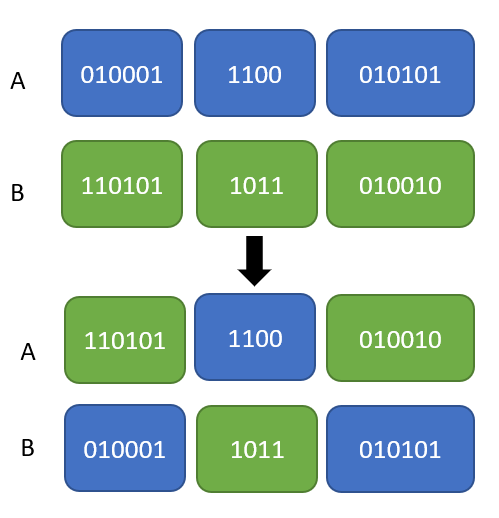
\includegraphics[height=8cm]{pic/TWO.PNG}}
		      \caption{多點交叉示意圖}
		      \label{fig:two}
	      \end{figure}

	\item
	      均勻交叉:
	      單點交叉跟多點交叉,存在染色體中某些部分的基因會被過早地捨棄,為了避免這個問題,有了均勻交叉,首先隨機選擇染色體上的交換位;然後隨機確定交換的基因是父輩染色體上交換位的前部分基因還是後部分基因;最後對父本染色體的基因進行重組從而產生新的下一代個體。如圖\ref{fig:avg}
	      \begin{enumerate}[(a)]
		      \item
		            隨機產生一個與個體長度相同的遮蔽字串(Mask String)W。

		      \item
		            若W=0則相對應父輩基因保留;若W=1則相對應父輩基因進行交叉。
	      \end{enumerate}
	      \begin{figure}[H]
		      \centerline{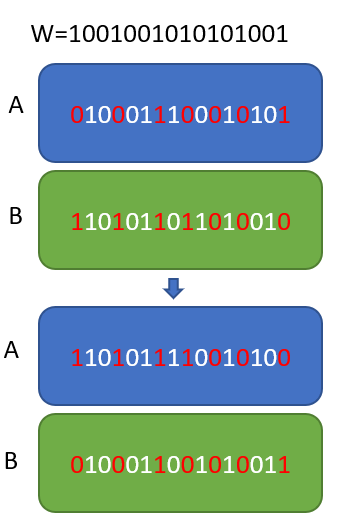
\includegraphics[height=8cm]{pic/AVG.PNG}}
		      \caption{均勻交叉示意圖W=1001001010101001}
		      \label{fig:avg}
	      \end{figure}


\end{enumerate}




\section{突變}
突變是為了避免種群中的染色體過於相似,使算法陷入區域極端,減慢或停止進化過程。遺傳算法利用交配操作從全局角度尋找一些較好的個體編碼結構,有助於獲得問題的最優解,但僅交配操作不能對搜索空間的細節進行局部搜索。這時,如果對個體編碼串中的一些基因值進行變異調整,個體可以從局部的角度更接近最優解,從而提高遺傳算法的局部搜索能力。突變示意圖\ref{fig:GAmut}

\begin{figure}[H]
	\centerline{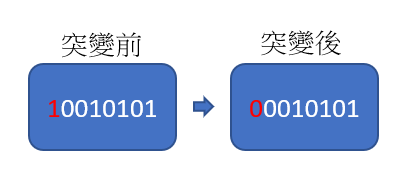
\includegraphics[height=5cm]{pic/GAmut.PNG}}
	\caption{突變示意圖}
	\label{fig:GAmut}
\end{figure}
